\documentclass[sigconf]{acmart}

\setcopyright{acmcopyright}

\acmDOI{xx.xxx/xxx_x}

\acmISBN{979-8-4007-0629-5/25/03}

%Conference
\acmConference[SAC'25]{ACM SAC Conference}{March 31 –April 4, 2025}{Sicily, Italy}
\acmYear{2025}
\copyrightyear{2025}

\acmArticle{4}
\acmPrice{15.00}

\begin{document}

\title{Energy consumption of C++ standard random number generators}
\subtitle{}

\renewcommand{\shorttitle}{Energy consumption of C++ standard random number generators}

\author{Ben Trovato}
\authornote{Boilerplate author names have been kept for double-blind review.}
\orcid{1234-5678-9012}
\affiliation{%
  \institution{Institute for Clarity in Documentation}
  \streetaddress{P.O. Box 1212}
  \city{Dublin}
  \state{Ohio}
  \country{USA}
  \postcode{43017-6221}
}
\email{trovato@corporation.com}

\renewcommand{\shortauthors}{B. Trovato}

\begin{abstract}
%La generación de números aleatorios es un asunto tan empleado como poco conocido en profundidad por sus usuarios. En este trabajo queremos adentrarnos en uno de estos campos poco conocidos: su consumo de energía. La mayoría de los trabajos sobre el tema suelen centrarse en el estudio de la calidad de los mismos o en medir sus tiempos de ejecución. Sin embargo, el consumo de energía es un aspecto crítico en la actualidad, especialmente en dispositivos móviles. En este trabajo hemos medido el consumo de energía de los generadores de números aleatorios estándar de C++. Los resultados muestran que existen amplias diferencias entre ellos en cuanto a consumo de energía, lo que puede ser relevante en aplicaciones que requieran de la generación de grandes cantidades de números aleatorios, tales como los algoritmos de aprendizaje y las metaheurísticas.
Random number generation is a widely used yet poorly understood topic among its users. In this paper, we aim to explore one of its lesser-known aspects: energy consumption. Most studies on the subject tend to focus on the quality of the generators or on measuring their execution times. However, energy consumption is a critical concern today, particularly for mobile devices. In this work, we have measured the energy consumption of standard C++ random number generators. The results show significant differences in energy usage between them, which could be relevant for applications that require the generation of large quantities of random numbers, such as learning algorithms and metaheuristics.
\end{abstract}

%
% The code below should be generated by the tool at
% http://dl.acm.org/ccs.cfm
% Please copy and paste the code instead of the example below.
%
\begin{CCSXML}
<ccs2012>
   <concept>
       <concept_id>10011007.10011074.10011075.10011079.10011080</concept_id>
       <concept_desc>Software and its engineering~Software design techniques</concept_desc>
       <concept_significance>300</concept_significance>
       </concept>
   <concept>
       <concept_id>10003752.10003809.10003716.10011136.10011797</concept_id>
       <concept_desc>Theory of computation~Optimization with randomized search heuristics</concept_desc>
       <concept_significance>300</concept_significance>
       </concept>
   <concept>
       <concept_id>10003752.10010061.10011795</concept_id>
       <concept_desc>Theory of computation~Random search heuristics</concept_desc>
       <concept_significance>500</concept_significance>
       </concept>
   <concept>
       <concept_id>10003752.10003809.10003716.10011136.10011797.10011799</concept_id>
       <concept_desc>Theory of computation~Evolutionary algorithms</concept_desc>
       <concept_significance>500</concept_significance>
       </concept>
   <concept>
       <concept_id>10011007.10010940.10010941.10010949.10010957.10010964</concept_id>
       <concept_desc>Software and its engineering~Power management</concept_desc>
       <concept_significance>500</concept_significance>
       </concept>
 </ccs2012>
\end{CCSXML}

\ccsdesc[300]{Software and its engineering~Software design techniques}
\ccsdesc[300]{Theory of computation~Optimization with randomized search heuristics}
\ccsdesc[500]{Theory of computation~Random search heuristics}
\ccsdesc[500]{Theory of computation~Evolutionary algorithms}
\ccsdesc[500]{Software and its engineering~Power management}

\keywords{Green computing, software engineering, evolutionary algorithms, genetic algorithms, energy-aware algorithms, random number generators}

\maketitle

\section{Introduction}
\label{sec:introduction}

%Los generadores de números pseudoaleatorios \cite{marsaglia2003random} son un recurso fundamental en computación. De ahí que hayan sido estudiados en prufundidad en multitud de trabajos. Sin embargo, la mayoría de estos trabajos se centran en la calidad de los números generados o en la eficiencia de los algoritmos que los generan. En este trabajo queremos centrarnos en un aspecto poco estudiado: el consumo de energía de los generadores de números aleatorios. Este aspecto es crítico en la actualidad, especialmente en dispositivos móviles, donde el consumo de energía es un factor limitante. En este trabajo hemos medido el consumo de energía de los generadores de números aleatorios estándar de C++.
Pseudo-random number generators \cite{marsaglia2003random} are a fundamental resource in computing, which is why they have been extensively studied in numerous works. However, most of these studies focus on the quality of the generated numbers or the efficiency of the algorithms that produce them. In this paper, we aim to focus on a less-studied aspect: the energy consumption of random number generators. This aspect is critical today, especially in mobile devices, where energy consumption is a limiting factor. In this work, we have measured the energy consumption of standard C++ random number generators.

%Su método general de funcionamiento se basa en el uso de una serie de semillas que se inicializan a un estado. Luego se aplica una función unidireccional sobre dichas semillas dando lugar a un número aleatorio. Para producir un nuevo número aleatorio, el último se usa como la nueva semilla y se somete al mismo proceso.
Most of them are initialized with a series of numbers used as seeds. A one-way function is then applied to these seeds, resulting in a random number. To generate a new random number, the previous one is used as the new seed and is subjected to the same process.

%Las propiedades de los generadores de números aleatorios pueden ser muy diversas según el ámbito en vayan a ser utilizadas. Para algunos de usos como la criptografía, los generadores deben pasar pruebas de calidad muy rigurosas tal como Diehard de Marsaglia \cite{marsaglia1997diehard}. Sin embargo, para otros muchos usos como los algoritmos genéticos, los generadores deben ser rápidos y eficientes aun a costa de su baja calidad. De hecho, algunos estudios sugieren que los algoritmos genéticos son poco sensibles a la calidad de los generadores de números aleatorios \cite{cardenas2011sensitiveness}.
The properties of random number generators can vary significantly depending on the field in which they are used. For certain applications, such as cryptography, generators must pass highly rigorous quality tests, such as Diehard \cite{marsaglia1997diehard} or TestU01 \cite{testu01}. However, for many other applications, such as genetic algorithms, the generators must be fast and efficient, even at the expense of lower quality. In fact, some studies suggest that genetic algorithms are not highly sensitive to the quality of random number generators \cite{cardenas2011sensitiveness}.

\section{Methodology}
\label{sec:methodology}

%Para poder medir el consumo de energía de los generadores de números aleatorios de C++ hemos escrito un programa que genera 100 millones de números aleatorios mediante cada uno de los generadores estándar de C++:
To measure the energy consumption of C++ random number generators, we wrote a program that generates 100 million random numbers using each of the C++ standard engines:
\begin{itemize}
    \item \texttt{std::knuth\_b}
    \item \texttt{std::minstd\_rand0} (\texttt{std::default\_random\_generator})
    \item \texttt{std::minstd\_rand}
    \item \texttt{std::mt19937} \cite{mersennetwister}.
    \item \texttt{std::mt19937\_64} \cite{mersennetwister}.
    \item \texttt{std::ranlux24\_base}
    \item \texttt{std::ranlux48\_base}
    \item \texttt{std::ranlux24} \cite{JAMES1994111}.
    \item \texttt{std::ranlux48} \cite{JAMES1994111}.
\end{itemize}

%También hemos añadido otros generadores bien conocidos por su interés, por su inclusión en otros lenguajes de programación o por formar parte del estado del arte:
We also included other well-known generators, either due to their relevance (\texttt{rand} de C), their inclusion in trendy programming languages like Rust and Zig, or their role in the state of the art:

\begin{itemize}
    \item \texttt{rand} de C.
    \item \texttt{mt11213b} \cite{mersennetwister}.
    \item \texttt{romutrio32} y \texttt{romutrio} \cite{overton2020romufastnonlinearpseudorandom}.
    \item \texttt{xoroshiro128+} \cite{blackman2021scrambled}.
    \item \texttt{xoshiro256+} \cite{blackman2021scrambled}.
\end{itemize}

%Para medir el consumo de energía hemos empleado perf \cite{perf} que permite hacerlo a través del estándar Running Average Power Limit (RAPL) \cite{rapl}. Cada programa se ha ejecuta 100 para obtener una precisión estadística razonable dentro de un sistema Fedora Linux con un procesador AMD Ryzen3 3100.
To measure energy consumption, we used perf \cite{perf}, which allows for this through the Running Average Power Limit (RAPL) standard \cite{rapl}. Each program was executed 100 times to obtain reasonable statistical accuracy on a Fedora Linux system with an AMD Ryzen3 3100 processor.

%Dado que perf solo es capaz de medir el consumo de energía de todo el sistema en conjunto hemos tenmido que recurrir a un pequeño truco para medir el consumo de energía de un único proceso. Hemos medido el consumo de nuestro programa y después hemos medido el consumo de la ejecución de la orden \texttt{sleep} durante el mismo tiempo que ha tardado nuestro programa en ejecutarse. La diferencia refleja el consumo de nuestro programa de forma aislada.

Since perf can only measure the energy consumption of the entire system as a whole, we implemented a specific methodology to isolate the energy consumption of a single process. Our approach involved two steps:

\begin{enumerate}
\item We measured the energy consumption of our program during its execution.
\item We then measured the energy consumption of the sleep command for a duration equal to our program's execution time.
\end{enumerate}

The difference between these two measurements provides an estimate of the isolated energy consumption of our program. This method allows us to differentiate between the baseline system energy consumption and the additional energy consumed by our specific process.

\section{Results}
\label{sec:results}

As can be seen from the results in Figure \ref{fig:pkg}, the energy consumption of the different generators varies significantly. The CPU time spent by the generators is also shown in Figure \ref{fig:cpu}. There is a clear correlation between energy consumption and CPU time, with the most efficient generators in terms of energy consumption also being the fastest.

\begin{figure}
\centering
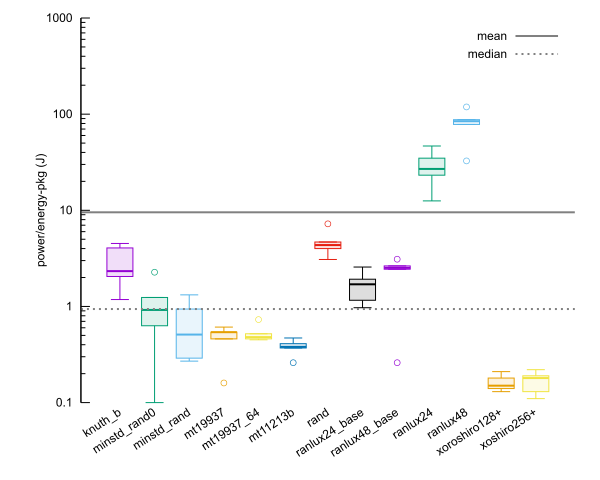
\includegraphics[width=\columnwidth]{pkg.png}
\caption{Energy consumption of C++ standard random number generators.}
\label{fig:cpu}
\end{figure}

\begin{figure}
\centering
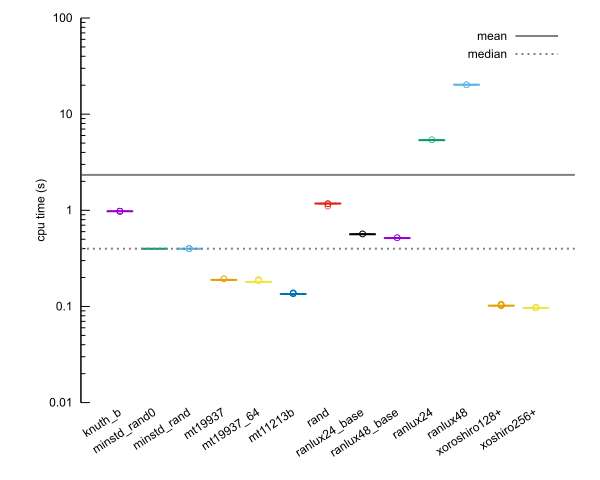
\includegraphics[width=\columnwidth]{cpu.png}
\caption{CPU time spent by C++ standard random number generators.}
\label{fig:pkg}
\end{figure}

% \begin{figure}
% \centering
% 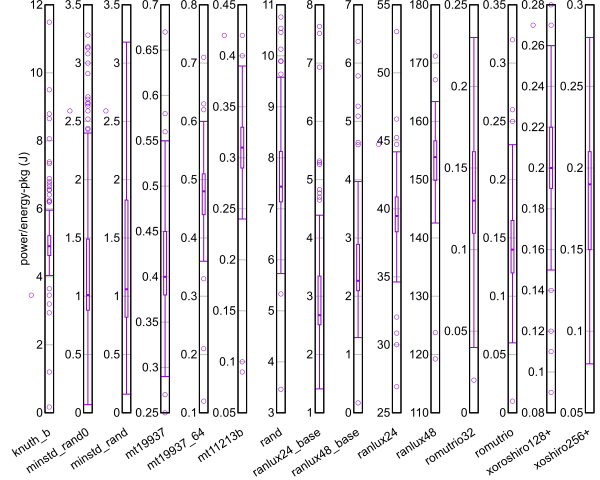
\includegraphics[width=\columnwidth]{all.png}
% \caption{Energy consumption of C++ standard random number generators.}
% \label{fig:all}
% \end{figure}

In our case, the 32 bits version of \texttt{romutrio}, \texttt{romutrio32}, is the most efficient in terms of energy consumption and CPU time, while the \texttt{ranlux48} generator is the least efficient. The differences between the generators are also reflected in Table \ref{tab:pkg}, which shows the means and standard deviations of the energy consumed and the CPU time spent by 100 runs of each engine creating 100 million random numbers. \texttt{romutrio32} consume the 0.09\% of the energy consumed by \texttt{ranlux48} and the 0.41\% of the CPU time spent by \texttt{ranlux48}.

\begin{table}
\centering
\caption{Means and standard deviations of energy consumption and CPU time of 100 runs of C++ standard engines when generating 100 million random numbers.}
\begin{tabular}{lcc}
\toprule
Generator & Energy (J) & Time (s) \\
\midrule
knuth\_b & 5.1256$\pm$1.4059 & 0.9778$\pm$0.0004 \\
minstd\_rand0 & 1.3238$\pm$0.7541 & 0.3985$\pm$\textbf{0.0002} \\
minstd\_rand & 1.3379$\pm$0.8194 & 0.3985$\pm$\textbf{0.0002} \\
mt19937 & 0.4116$\pm$0.0693 & 0.1891$\pm$0.0007 \\
mt19937\_64 & 0.4770$\pm$0.0759 & 0.1806$\pm$0.0019 \\
mt11213b & 0.3068$\pm$0.0482 & 0.1349$\pm$0.0006 \\
rand & 7.6998$\pm$1.1038 & 1.1750$\pm$0.0075 \\
ranlux24\_base & 3.0864$\pm$1.1094 & 0.5636$\pm$0.0013 \\
ranlux48\_base & 2.5486$\pm$0.9063 & 0.5145$\pm$0.0009 \\
ranlux24 & 39.5458$\pm$3.1765 & 5.3631$\pm$0.0193 \\
ranlux48 & 153.1331$\pm$6.6647 & 20.2619$\pm$0.0232 \\
romutrio32 & \textbf{0.1357}$\pm$0.0340 & \textbf{0.0826}$\pm$0.0004 \\
romutrio & 0.1415$\pm$0.0405 & 0.0848$\pm$0.0005 \\
xoroshiro128+ & 0.2037$\pm$\textbf{0.0313} & 0.1021$\pm$0.0005 \\
xoshiro256+ & 0.1817$\pm$0.0379 & 0.0968$\pm$\textbf{0.0002} \\
\bottomrule
\end{tabular}
\label{tab:pkg}
\end{table}

After \texttt{romutrio32} and \texttt{romutrio}, the next best engines are the Mersenne Twister \texttt{mt11213b} and XOR based ones from Marsaglia, \texttt{xoroshiro128+}, and \texttt{xoshiro256+}, though not by a large margin.

Is also important to note that most of the implementations with lower energy consumption are 32 bits based, although their corresponding 64 bits versions are not much worse. As we can see when comparing a couple of examples:
\begin{itemize}
\item \texttt{mt19937\_64}, the 64 bits version of \texttt{mt19937}, consumes 15.89\% more energy and -4.49\% less CPU time.
\item \texttt{romutrio}, the 64 bits version of \texttt{romutrio32}, consumes 4.27\% more energy and 2.66\% less CPU time.
\end{itemize}

The energy consumption of the classic C \texttt{rand} generator is also very high, which is consistent with its poor performance in terms of CPU time. In spite of being one of the 32 bits implementations.

As a curious case, we can highlight \texttt{mt11213b}, one of the Mersenne Twister family generators. Its characteristics are among the best, and the only thing that differentiates it from \texttt{mt19937} is the set of constants and initial seeds. However, \texttt{mt11213b} consumes 34.16\% less energy and 40.18\% less CPU time than \texttt{mt19937}.

After \texttt{romutrio32} and \texttt{romutrio}, the next best engines are the Mersenne Twister \texttt{mt11213b} and the XOR-based ones from Marsaglia, \texttt{xoroshiro128+} and \texttt{xoshiro256+}, though the differences are not significant.

It is also important to note that most of the implementations with lower energy consumption are 32-bit based, although their corresponding 64-bit versions are not much worse. This can be observed in the following comparisons:

\begin{itemize}
    \item \texttt{mt19937\_64}, the 64-bit version of \texttt{mt19937}, consumes 15.89\% more energy and uses 4.49\% less CPU time.
    \item \texttt{romutrio}, the 64-bit version of \texttt{romutrio32}, consumes 4.27\% more energy and uses 2.66\% less CPU time.
\end{itemize}

The energy consumption of the classic C \texttt{rand} generator is also very high, which is consistent with its poor performance in terms of CPU time, despite being one of the 32-bit implementations.

A notable case is \texttt{mt11213b}, one of the Mersenne Twister family generators. Its characteristics are among the best, and the only difference between it and \texttt{mt19937} is the set of constants and initial seeds. However, \texttt{mt11213b} consumes 25.46\% less energy and 28.66\% less CPU time than \texttt{mt19937}.


\section{Conclusions}
\label{sec:conclusions}

las conclusiones......

\begin{acks}
Hidden for double-blind review
\end{acks}

\bibliographystyle{ACM-Reference-Format}
\bibliography{std-sac-poster-2025}

\end{document}
